% -*- TeX-engine: default; -*-
\documentclass[10pt,sigconf,anonymous]{acmart}
\usepackage[font=footnotesize]{subcaption}
\usepackage[utf8]{inputenc}
\usepackage[T1]{fontenc}
\usepackage{url}
\usepackage{booktabs}
\usepackage{xcolor}
\usepackage{enumitem}
\usepackage{algorithm}
\usepackage[noend]{algpseudocode}

\setcopyright{none}
\acmYear{2018}
\copyrightyear{2018}
\acmConference[CoNEXT'18]{ACM CoNEXT 2018}{December 2018}{Heraklion/Crete, Greece}
\settopmatter{printccs=false,printacmref=false}
\widowpenalty=100
\clubpenalty=100
\brokenpenalty=100

\begin{document}
\title{The eXpress Data Path: Fast Programmable Packet Processing in the
  Operating System Kernel}
\author{Toke Høiland-Jørgensen}
\affiliation{%
  \institution{Karlstad University}}
\email{toke.hoiland-jorgensen@kau.se}

\author{Jesper Dangaard Brouer}
\affiliation{%
  \institution{Red Hat}}
\email{brouer@redhat.com}

\author{Daniel Borkmann}
\affiliation{%
  \institution{Cilium.io}}
\email{daniel@cilium.io}

\author{John Fastabend}
\affiliation{%
  \institution{Cilium.io}}
\email{john@cilium.io}

\author{Tom Herbert}
\affiliation{%
  \institution{Quantonium Inc.}}
\email{tom@herbertland.com}

\author{David Ahern}
\affiliation{%
  \institution{Cumulus Networks}}
\email{dsahern@gmail.com}

\author{David Miller}
\affiliation{%
  \institution{Red Hat}}
\email{davem@redhat.com}

\renewcommand{\shortauthors}{T. Høiland-Jørgensen et al.}
\renewcommand{\shorttitle}{The eXpress Data Path}
\captionsetup{font+=small}

\begin{abstract}
  % Max abstract length is 200 words
  Programmable packet processing is most often implemented using kernel bypass
  techniques, where a userspace application takes complete control of the
  networking hardware to avoid expensive context switches between kernel and
  userspace. However, in this model the processing application has to either
  perform cumbersome re-injection of packets into the kernel, or handle all
  network traffic itself, making fast packet processing an all-or-nothing
  proposition.

  To overcome this limitation, we propose a novel approach to programmable
  packet processing where the operating system kernel itself provides a safe
  execution environment for custom packet processing applications, executed in
  device driver context. This system, called the eXpress Data Path (XDP), has
  been merged into the mainline Linux kernel and provides a fully integrated
  solution working in concert with the kernel's network stack. In XDP,
  applications written in higher level languages such as C are compiled into
  custom bytecode which the kernel statically analyses for safety, and
  translates into native instructions.

  We show that XDP achieves single-core packet processing performance as high as
  25 million packets per second, and illustrate the flexibility of the
  programming model through three example use cases: layer-3 routing, inline
  DDoS protection and layer-4 load balancing.
\end{abstract}

% TODO: Add ccsxml tags and update keywords

\keywords{XDP, BPF, Programmable Networking}
\maketitle

\section{Introduction}%
\label{sec:introduction}
High-performance packet processing in software has very tight bounds on the time
spent processing each packet ($\simeq6$~ns per packet at 100 Gbps). Network
stacks in general purpose operating systems are typically optimised for
flexibility, trading off performance by performing too many operations per
packet to be able to keep up with these high packet rates. This has led to the
increased popularity of special-purpose toolkits for software packet processing,
such as the Data Plane Development Kit (DPDK)~\cite{dpdk}. Such toolkits
generally bypass the operating system completely, instead passing control of the
network hardware directly to the network application and dedicating one, or
several, CPU cores exclusively to packet processing.

The kernel bypass approach can significantly improve performance, but has the
drawback that it is more difficult to integrate with the existing networking
stack, and applications have to re-implement a great deal of functionality
otherwise provided by the operating system kernel. In the worst case, this leads
to the need to operate two separate stacks; one to perform high-speed packet
processing and one to run normal application or container workloads, resulting
in increased systems complexity, management and maintainability costs, and at
the same time blur strict security boundaries otherwise provided by the
operating system kernel. The latter is in particular problematic as today's
infrastructure is moving towards container-based workloads coupled with
orchestration systems such as Docker or Kubernetes, where the kernel plays a
dominant role in resource abstraction and isolation.

As an alternative to the all-or-nothing kernel bypass packet processing
technique, we present a system that adds programmability directly in the
operating system networking stack in a cooperative way, making it possible to
perform high-speed packet processing that integrates seamlessly with existing
systems, while selectively leveraging functionality in the operating system.
This framework, called the eXpress Data Path (XDP), works by defining a limited
execution environment in the form of a virtual machine running a custom bytecode
that is based on an extended version of the Berkeley Packet Filter. This
environment executes custom programs directly in the device driver context,
before the kernel performs any other packet processing tasks. The kernel ensures
safety and performance by statically verifying the program before it is loaded,
and dynamically compiles the virtual machine bytecode into native machine
instructions.

XDP has been gradually integrated into the Linux kernel over several releases,
but no complete architectural description of the system as a whole exists in the
literature. In this work we present such a high-level design description of XDP,
its capabilities and how it integrates with the rest of the Linux kernel. Our
performance evaluation shows raw packet processing performance of up to 25
million packets per second per CPU core, which does not quite match the highest
achievable performance in a DPDK-based application on the same hardware.
However, we argue that the remaining performance gap is quite feasible to close
using the current XDP architecture. And, more importantly, the XDP system offers
several compelling advantages over DPDK and other kernel bypass solutions.
Specifically, XDP:

\begin{itemize}
\item Integrates cooperatively with the regular networking stack, retaining full
  control of the hardware in the kernel. This means that the kernel security
  boundary is intact, and no changes to network configuration and management
  tools are needed. In addition, any network adapter with a Linux driver can be
  supported by XDP; no special hardware features are needed.

\item Makes it possible to selectively utilise kernel network stack features
  such as the routing table, keeping the same configuration interface, while
  accelerating the critical performance paths.

\item Provides a stable programming interface for packet processing
  applications, which carries the same stability guarantees as every other
  kernel interface.

\item Is completely transparent to applications running on the host, enabling
  new deployment scenarios such as inline DDoS protection on application
  servers.

\item Can be dynamically re-programmed without service interruption, which means
  that features can be removed completely when they are not needed, and programs
  can react to conditions in other parts of the kernel as well as events from
  userspace.

\item Does not require dedicating full CPU cores to packet processing, which
  means lower traffic levels translates directly into lower CPU usage. This has
  important efficiency and power saving implications.
\end{itemize}

In the rest of this paper we present the design of XDP and our performance
analysis. This is structured as follows: Section~\ref{sec:related-work} first
outlines related work. Section~\ref{sec:design} then presents the design of the
XDP system and Section~\ref{sec:perf-eval} presents our evaluation of its raw
packet processing performance. Section~\ref{sec:usecases} supplements this with
examples of real-world use cases that can be implemented with XDP. Finally,
Section~\ref{sec:limitations} presents some known limitations of XDP and future
work to address them, and Section~\ref{sec:conclusion} concludes.

\section{Related Work}%
\label{sec:related-work}

Programmable packet processing continues to gain momentum as the performance
attainable on commodity hardware rises, and costs fall. Programmable hardware
devices such as the NetFPGA~\cite{lockwood2007netfpga}, allows this processing
to continue to happen on specialised hardware, by exposing an API that makes it
possible to run arbitrary packet processing tasks on the FPGA-based dedicated
hardware. The P4 language~\cite{bosshart2014p4} seeks to extend this
programmability to a wider variety of packet processing hardware.

However, even though specialised hardware has begun to gain data plane
programmability, the flexibility of common off-the-shelf (COTS) hardware has
obvious advantages, and as performance increases and cost decreases, packet
processing systems running on COTS hardware become ever more common. These
include applications performing single functions, such as
switching~\cite{rizzo2012vale}, routing~\cite{han2010packetshader}, named-based
forwarding~\cite{kirchner2016augustus}, classification~\cite{santiago2012wire},
caching~\cite{mansilha2015hierarchical} or traffic
generation~\cite{emmerich2015moongen}. They also include more general solutions
which are highly customisable and can operate on packets from a variety of
sources~\cite{han2012megapipe,marian2012netslices,linguaglossa2017high,morris1999click,dobrescu2009routebricks}.

The applications listed above are all higher level applications or frameworks
focused on implementing specific packet processing applications, or classes
thereof. Whereas XDP is a lower-level framework that focuses on how to build a
high-performing base for packet processing applications to run on. To achieve
such high performance on COTS hardware, it is necessary to remove any
bottlenecks between the networking interface card (NIC) and the program
performing the packet processing. Since one of the main sources of performance
bottlenecks is the interface between the operating system kernel and the
userspace applications running on top of it (because of the high overhead of a
system call), low-level packet processing frameworks have to manage this
overhead in one way or another. The approaches taken fall into three broad
categories: (a) implementing parts of the application as a module inside the
kernel itself, (b) providing an interface for userspace to access packet data
with lower overhead than with traditional sockets, or (c) bypassing the kernel
entirely and handing over control of the networking device directly to
userspace.

In the first category, systems such as the OpenVswitch~\cite{openvswitch}
virtual switch and the Click~\cite{morris1999click} virtual router framework
provide kernel modules that offload part of their functionality into the kernel.
These are implemented as loadable kernel modules that provide configuration APIs
to userspace, but performs packet processing directly in the kernel. The
drawback of implementing packet processing applications in this way, is that it
requires deep familiarity with internal kernel APIs, and a failure of the
network processing application in most cases leads to a failure of the entire
system. In addition, such systems generally integrate into the kernel networking
stack, which means that the overhead of the network stack processing itself is
retained.

In the second category, various systems introduce kernel modules that do not
perform packet processing themselves, but instead focus on moving packet data
out to userspace with as little overhead as possible, typically via shared
memory. This allows the packet processing application to operate in userspace
with no risk of crashing the system. Examples of this approach include
PF\_RING~\cite{deri2009modern}, the Packet I/O engine that is part of
PacketShader~\cite{han2010packetshader}, the Netmap~\cite{rizzo2012netmap}
framework, as well as special-purpose operating systems as
Arrakis~\cite{peter2016arrakis} and ClickOS~\cite{martins2014clickos}. The
drawback of this approach is that it requires extensive changes to the operating
system. In addition, even if the frameworks mentioned above improve performance
significantly, they still lack behind in performance compared to kernel bypass
solutions~\cite{gallenmuller_comparison_2015}.

In the third category of kernel bypass techniques, we find the PF\_RING ZC
module~\cite{pfringzc}, the hardware-specific Solarflare
OpenOnload~\cite{openonload} and, most prominently, the DataPlane Development
Kit (DPDK)~\cite{dpdk}, which started out as an Intel-specific hardware support
package, but has since seen a wide uptake under the stewardship of the Linux
Foundation. This approach offers excellent performance, but has the drawback
that it is more difficult to integrate with the rest of the system, as mentioned
in the introduction.

XDP takes the first approach to lowering overhead, and places the packet
processing in kernel device driver context, before any other processing. This
means that not only the overhead of passing every packet to userspace is
avoided, but also the overhead of the regular kernel networking stack. By using
a custom byte code format for the programming, which can be statically verified
to not adversely affect the functioning of the rest of the kernel, most of the
fragility issues normally faced by in-kernel packet processing implementations
are avoided. In addition, the byte code format and execution context are part of
the kernel Application Binary Interface (ABI) to userspace, which means that the
usual ABI stability guarantees apply; and so application do not have to keep up
with future changes in the kernel to be able to continue to function.

While XDP is primarily an instance of the first of the three approaches mentioned
above, it also borrows aspects from the other two: For applications that prefer
receiving the full packet contents in userspace, XDP also contains features that
offer higher performance when redirecting packets to applications, virtual
machines and containers running in userspace. This include the ability to bypass
parts of the network stack processing, and even to perform zero-copy transfer of
packets to userspace applications using a special socket type. These facilities
roughly correspond to the second approach mentioned above. Finally, XDP applies
some of the same performance enhancing techniques used by the kernel bypass
frameworks, such as packet batching and the ability to process packets
immediately after they are received from the hardware.

\section{The design of XDP}
\label{sec:design}
XDP is designed to integrate with the Linux networking stack, making it possible
to take advantage of the extensive feature set of the operating system, while
adding custom packet processing as required. This section describes how these
parts of XDP work, and how they fit together to create the full system. The
major components of the XDP system are:

\begin{itemize}
\item \textbf{The XDP driver hook} is the main entry point for an XDP program,
  and is executed as soon as a packet is received from the hardware.

\item \textbf{The eBPF virtual machine} executes the byte code of the XDP
  program, and just-in-time-compiles it for added performance.

\item \textbf{The eBPF verifier} statically verifies programs before they are
  loaded to make sure they do not crash or corrupt the running kernel.

\item \textbf{BPF maps} are key/value stores that serve as the primary
  communication channel to the rest of the system.
\end{itemize}

\begin{figure}[t]
\centering
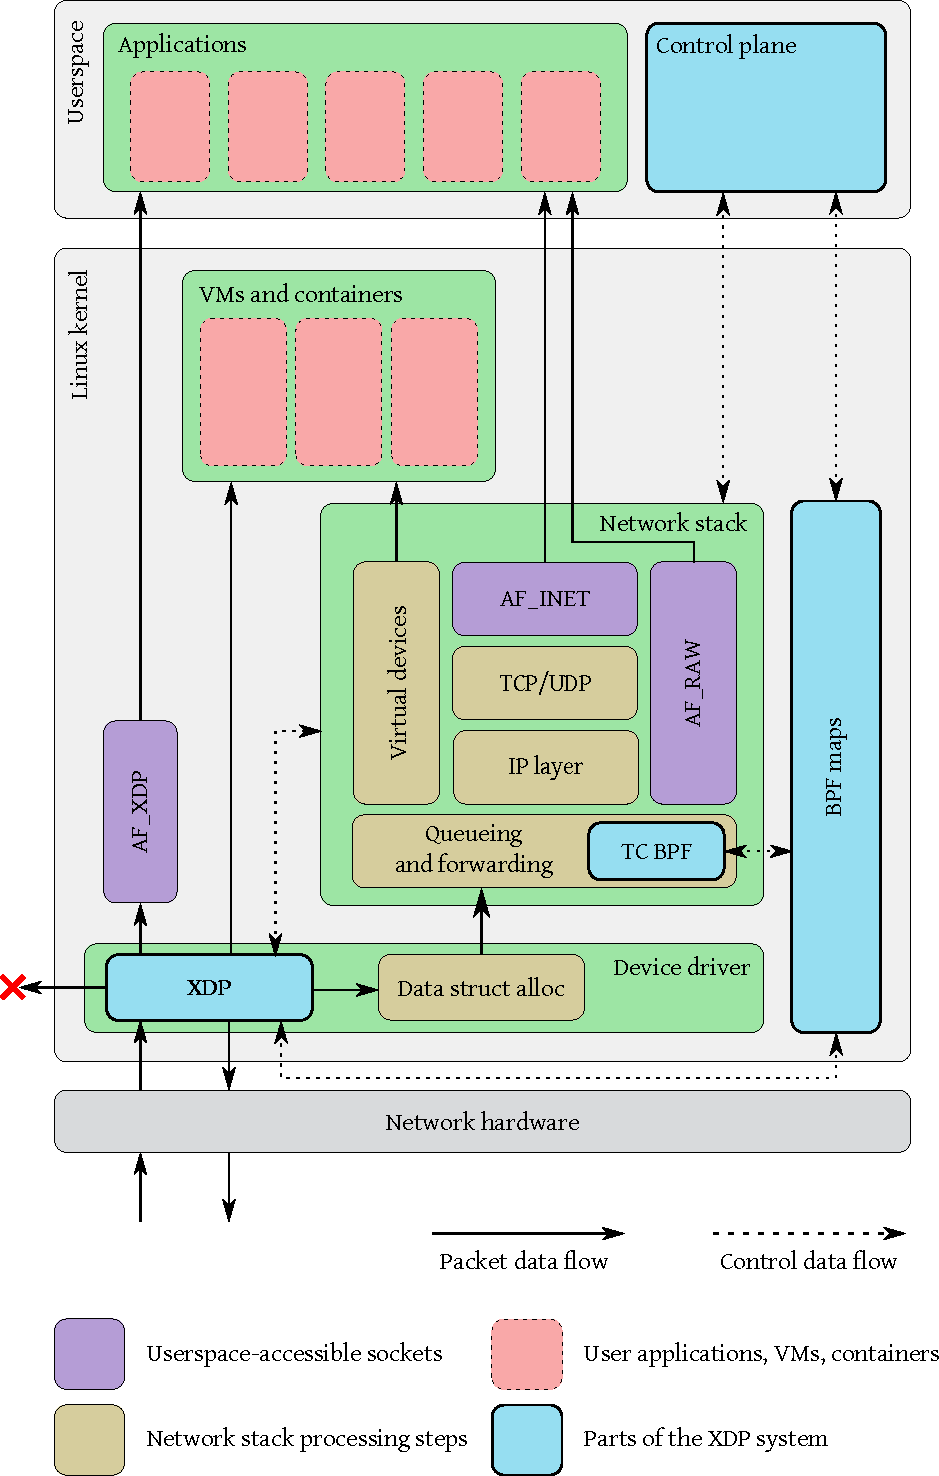
\includegraphics[width=\linewidth]{figures/kernel-diagram.pdf}
\caption{\label{fig:xdp-kernel} XDP's integration with the Linux network stack.}
\end{figure}


We describe each of these components below. Figure~\ref{fig:xdp-kernel} shows a
diagram of how XDP integrates into the Linux kernel, and
Figure~\ref{fig:xdp-execution} shows the execution flow of a typical XDP
program. Together, they give an overview of the XDP system, and they will be
referenced throughout the exposition below.

\subsection{The XDP Driver Hook}
\label{sec:prog-model}

\begin{figure*}[t]
\centering
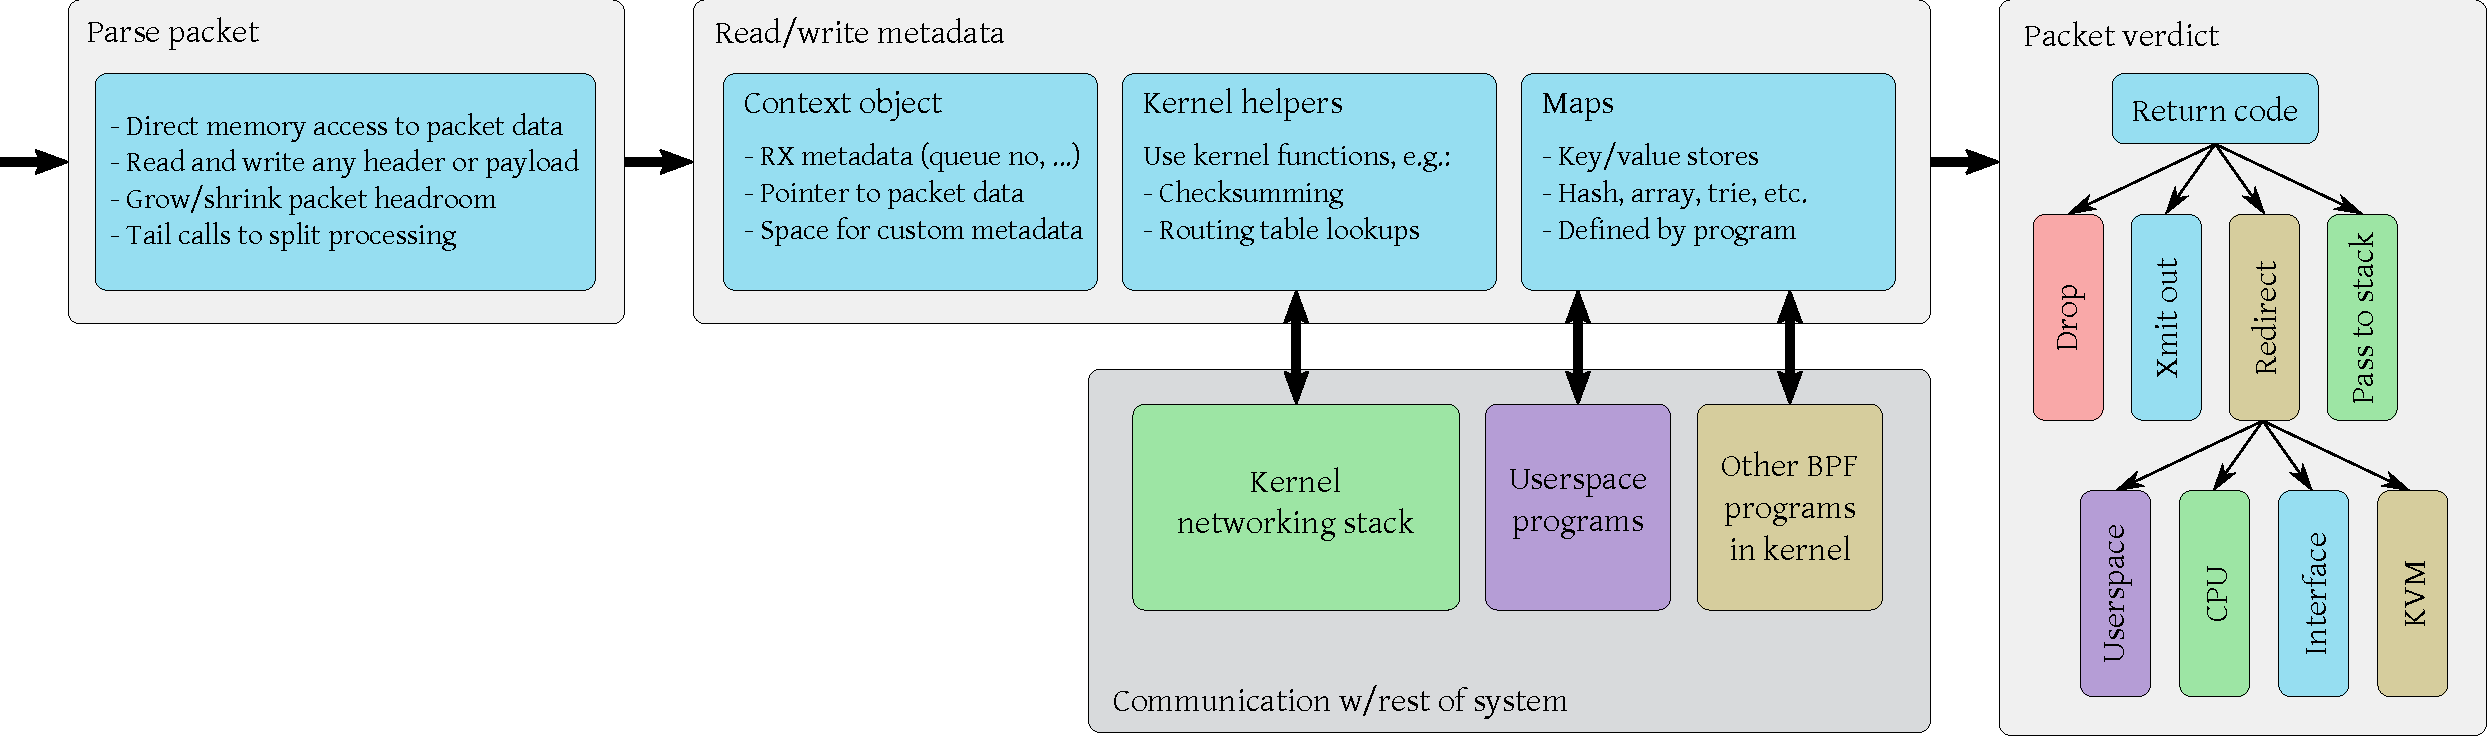
\includegraphics[width=\linewidth]{figures/xdp-execution-diagram.pdf}
\caption{\label{fig:xdp-execution} Execution flow of a typical XDP program. When
  a packet arrives, the program starts by parsing packet headers to extract the
  information it will react on. Based on this, combined with information from
  one or more of the metadata facilities, a packet can be rewritten and a final
  verdict for the packet determined. The program can alternate between packet
  parsing, metadata lookup and rewriting, all of which are optional. The final
  verdict is given in the form of a program return code.}
\end{figure*}


An XDP program is run by a hook in the network device driver when a packet
arrives, and so is entirely event-driven. The program is executed directly in
context of the device driver, without context switching to userspace. As shown
in Figure~\ref{fig:xdp-kernel}, the program is executed at the earliest possible
moment after a packet is received from the hardware, before the kernel allocates
its per-packet \emph{sk\_buff} data structure or performs any parsing of the
packet. This allows for high performance, but the program has to parse raw
packet data itself.

Figure~\ref{fig:xdp-execution} shows the various processing steps typically
performed by an XDP program. The program starts its execution with access to a
pointer to a context object. This object contains pointers to the raw packet
data (direct packet access bounds are checked by the verifier), along with
metadata fields describing which interface and receive queue the packet came in
on, etc.

The program typically begins by parsing packet data, and can pass control to a
different XDP program through tail calls, thus splitting processing into
logical sub-units (based on, say, IP header version).

After parsing the packet data, the XDP program can read or write metadata
associated with the packet itself, or available in other parts of the operating
system. The former is accessible through the context object, which contains a
pointer to a special memory area is available for XDP to store arbitrary
metadata that will be available to other XDP programs, as well as to other parts
of the kernel and userspace. In addition to this, an XDP program also has access
to kernel facilities that provide helper functions and additional metadata.
These allow the XDP program to gather additional metadata through helper
functions and maps (dotted lines in Figure~\ref{fig:xdp-kernel} and the top part
of Figure~\ref{fig:xdp-execution}). New helpers are actively been added by the
kernel development community in response to user requests, continuously
expanding the functionality that XDP programs can make use of.

Finally, the program can write any parts of the packet data buffer, including
expanding or shrinking the packet to add or remove headers. This allows it to
perform encapsulation or decapsulation, as well as, for instance, rewrite
address fields for forwarding. Various kernel helpers are available to assist in
things like checksum calculation for a modified packet.

These three steps (reading, metadata processing, and writing packet data)
correspond to the light grey boxes on the left side of
Figure~\ref{fig:xdp-execution}. Since XDP programs can contain arbitrary
instructions, the different steps can alternate and repeat in arbitrary ways.
However, to achieve high performance, it is generally necessary to structure the
execution order as described here.

Similar to a regular userspace program, an XDP program ends its execution with a
return code, instructing the kernel what to do with the packet. This is shown on
the right-hand side of the figure. There are three simple return codes which
either drops the packet, immediately re-transmits it out the same network
interface, or allows the packet to be processed by the kernel networking stack.
In addition to these simple actions, the XDP program can \emph{redirect} the
packet, which controls its further processing.

The redirect facility is designed as a flexible forwarding mechanism, which can
be extended with new redirect targets without changing the driver code. This is
achieved by using BPF maps to store the redirect targets, which also allows
these targets to be dynamically updated from userspace. Currently, redirecting
can be used (1) to transmit the raw packet out a different network interface
(including virtual interfaces which are connected to virtual machines), (2) to
pass it to a different CPU for further processing, or (3) to pass it directly to
a special userspace socket address family (\texttt{AF\_XDP}). These different
packet paths are shown as solid lines in Figure~\ref{fig:xdp-kernel}.

\subsection{The eBPF Virtual Machine}
\label{sec:bpf-vm}
The eBPF virtual machine is an evolution of the original BSD packet filter (BPF)
\cite{mccanne_bsd_1993} which has seen extensive use in various packet filtering
applications over the last decades. BPF uses a register-based virtual machine to
describe filtering actions. The original virtual machine has two 32-bit registers and
understands 22 different instructions. This makes BPF well-suited for packet
filtering operations, but limited as a general purpose virtual machine. eBPF
extends the original BPF virtual machine to allow full general purpose execution
and efficient just-in-time (JIT) compilation into native machine code. Support
for compiling (restricted) C code into eBPF is included in the LLVM compiler
suite.

The verifier (described in the next section) ensures that user-supplied programs
cannot harm the running kernel. With this in place, it is safe to execute the
code directly in the kernel address space, which makes eBPF useful for a wide
variety of tasks in the Linux kernel. Apart from the XDP driver hook, this
includes packet processing in the Traffic Control (TC) subsystem, where eBPF
programs can filter packets after they have been parsed by the kernel, or before
they are passed to the hardware from applications. This is marked as ``TC BPF''
in Figure~\ref{fig:xdp-kernel}. In addition, eBPF programs can be attached to
various places in the kernel that are unrelated to networking (not shown in the
figures). These include \emph{cgroups}, which control resource usage for groups
of processes (used for implementing containers on Linux, for instance), as well
the \emph{tracepoint} and \emph{kprobe} introspection subsystems which allow
attaching eBPF programs to arbitrary kernel functions. Because all eBPF programs
can share the same set of maps, this makes it possible for programs to react to
arbitrary events in other parts of the kernel. For instance, and XDP program
could drop packets if processing load increases above a certain threshold.

At the instruction set level, eBPF extends the original BPF virtual machine by
adding more registers and more instructions. The number of registers is
increased from two to eleven (numbered \texttt{R0}--\texttt{R10}, where
\texttt{R10} is reserved for a read-only frame pointer), and register widths are
increased to 64 bits, with 32-bit sub-registers accessible through certain
instructions to provide compatibility with classic BPF programs. The 64-bit
registers map one-to-one to hardware registers on all 64-bit architectures
supported by the kernel, which eases JIT compilation.

The added instructions are primarily arithmetic and logic instructions that
allows efficient manipulation of the larger register sizes. In addition to this,
eBPF adds a \emph{call} instruction for function calls, and adopts the same
calling convention as the C language conventions used on the architectures
supported by the kernel. Along with the register mapping mentioned above, this
makes it possible to map a BPF call instruction to a single native call
instruction, enabling function calls with close to zero additional overhead.
This facility is used by eBPF to support helpers that eBPF programs can call to
interact with the kernel while processing, as well as for function calls within
the same eBPF program. A special case of function calls are tail calls, which
replaces the running eBPF program with the target of the call. This can be used
to split up processing into logical sub-parts, where execution is dispatched to
subsequent parts and never returns to the caller.

A BPF program starts its execution with \texttt{R1} containing a pointer to a
\emph{context} object, the contents of which varies with the type of program. As
explained above, for XDP programs the context object is a structure that allows
the BPF program to access the packet data itself, as well as various items of
metadata, including space for arbitrary data that is carried along with the
packet and is accessible by other BPF programs that operate on the packet at
later stages of processing.

Finally, the eBPF virtual machine supports dynamically loading and re-loading
programs, and the kernel manages the life cycle of all programs. Combined with
dynamic dispatch to other programs using tail calls, this makes it possible to
limit the amount of processing actually performed for a given situation, and
also to dynamically update how processing is performed. This also makes it
possible to dynamically compile programs with hard-coded values derived from
configuration, avoiding expensive data structure lookups for common tasks.

\subsection{The eBPF Verifier}
\label{sec:bpf-verifier}
As mentioned in the previous section, eBPF code runs directly in the kernel
address space, which means that it can directly address, and potentially
corrupt, arbitrary kernel memory. To prevent this from happening, the kernel
enforces a single entry point for loading all BPF programs (through the
\texttt{bpf()} system call). When loading a BPF program it is first analysed by
the in-kernel eBPF verifier. The verifier performs a static analysis of the
program byte code to ensure that the program performs no actions that are unsafe
(such as accessing arbitrary memory), and that the program will terminate. The
latter is ensured by disallowing loops and limiting the maximum program
size.\footnote{Verifying termination of arbitrary programs (that are not limited
  in this way) implies solving the halting problem, which we consider to be out
  of scope for this work.} The verifier works by first building a directed
acyclic graph (DAG) of the control flow of the program. This DAG is then
verified as follows:

\begin{table}[tbp]
\caption{\label{tbl:vrf-state-vars}
eBPF verifier state variables}
\centering
\begin{tabular}{ll}
\toprule
Variable & Contains\\
\midrule
\texttt{type} & One of the types in Table \ref{tbl:reg-types}\\
\texttt{id} & ID for tracking copies of same variable\\
\texttt{fixed\_offset} & Pointer offset (after arithmetic)\\
\texttt{range\_unsigned} & Min and max values (unsigned)\\
\texttt{range\_signed} & Min and max values (signed)\\
\texttt{tnum} & Mask and value of known bits\\
\bottomrule
\end{tabular}
\end{table}

First, the verifier performs a depth-first search on the DAG to ensure it
contains no loops (no backwards jumps) and that it contains no unsupported or
unreachable instructions. Then, in a second pass, the verifier walks all
possible paths of the DAG while tracking the state of all registers. The purpose
of this second pass is to ensure that the program performs only safe memory
accesses, and that any helper functions are called with the right argument
types. This is ensured by rejecting programs that perform load or call
instructions with invalid arguments. Argument validity is determined by tracking
the state of all registers and stack variables through the execution of the
program, as explained in the following.

\subsubsection{Register state tracking}
\label{sec:reg-state}
To track data access, the verifier assigns five state variables to each
register, listed in Table~\ref{tbl:vrf-state-vars}, with the possible types listed in
Table~\ref{tbl:reg-types}. The fixed offset is used to track the result of pointer
arithmetic with fixed values, while the ranges and \emph{tnum} are used to track
variable offsets of pointers, as well as the ranges of scalar variables.

\begin{table}[tbp]
\caption{\label{tbl:reg-types}
eBPF verifier type annotations. The last column indicates whether pointer arithmetic is allowed for this type of pointer.}
\centering
\begin{tabular}{lll}
\toprule
\multicolumn{3}{c}{\textbf{Non-pointer types}} \\
Name & Meaning \\
\midrule
\texttt{NOT\_INIT}            & Not initialised         \\
\texttt{SCALAR\_VALUE}        & Any numerical value       \\
\midrule
\multicolumn{3}{c}{\textbf{Pointer types}} \\
Name & Pointing to & Arithm\\
\midrule
\texttt{CTX}                  & Context              & Yes \\
\texttt{MAP}                  & BPF map              & No  \\
\texttt{MAP\_VALUE}           & Value in map         & Yes \\
\texttt{MAP\_VALUE\_OR\_NULL} & Value in map or NULL & No  \\
\texttt{STACK}                & Stack frame          & Yes \\
\texttt{PACKET}               & Packet data start    & Yes \\
\texttt{PACKET\_END}          & Packet data end      & No  \\
\bottomrule
\end{tabular}
\end{table}

At the beginning of the program, \texttt{R1} contains a pointer to the execution
context, and its type is a \texttt{CTX} pointer; \texttt{R10} is a \texttt{STACK}
pointer, and all other registers are \texttt{NOT\_INIT}. At each execution step,
register states are updated based on the operations performed by the program.
When a new value is stored to a register, it inherits the state variables of the
source of the value. Arithmetic operations on scalar values will affect the
value of the \emph{tnum} state variable, which tracks which bits in a register
are known, and their value. The \emph{tnum} is a pair of \emph{mask}, which
contains the bits whose value is unknown, and a \emph{value} which contains the
bits that are known to be set to 1. Load operations set these, for instance
loading a byte from memory will result in the top 56 bits being known to be
zero, and the bottom 8 bits to be unknown. Arithmetic updates these values
according to their operation.

Branches in the instruction tree will update the register state according to the
logical operation contained in the branch. For example, a comparison "\texttt{R1
  > 10}" compare will set the maximum value of \texttt{R1} to 10 in one branch,
and the minimum value to 11 in the other. If a comparison is performed with a
scalar value rather than a constant, the knowledge of which bits are set is used
to compute the ranges for the branches (using the minimum and maximum possible
values of unknown bits as appropriate). Finally, a branch that checks whether
register with a \texttt{MAP\_VALUE\_OR\_NULL} pointer is different from
\texttt{NULL} will turn that register into a pointer with type
\texttt{MAP\_VALUE} in the \emph{true} branch, which makes it possible to
derefence the pointer.

Using the information contained in the state variables, it is possible for the
verifier to predict the ranges of memory that it is possible for each load
instruction to access. It uses this information to ensure that only safe memory
accesses are performed. Any eBPF program that makes memory accesses that the
verifier cannot prove are safe are simply rejected at load time. The verifier
also uses the range information to enforce aligned memory accesses.

For pointers to context objects, the execution context of the eBPF program
indicates allowed memory offsets for their context objects through a callback
performed by the verifier. For map values, the map definition defines the size
of the values, which is used to bound the allowed memory accesses. For pointers
to stack values, only ranges previously stored on the stack are valid. And
finally, for pointers to packet data, only ranges known to be less than the
packet length are allowed. The latter is enforced by ensuring that the program
makes appropriate range checks through comparison with the special
\texttt{PACKET\_END} pointer that is included in the context structure. This
approach means that the program can be statically verified to make safe length
checks on the variable-length packet data, which enables program instructions to
directly access packet data. This is an important reason for the high
performance of eBPF programs that are used for packet processing, as they are in
XDP.

When pointers are copied to other registers, a bounds check on one copy can be
used to infer the valid ranges of the other copies, even after the copy
occurred. The \emph{id} state variable is used for this purpose for packet access and
map value pointers. For packet access, all pointers with the same variable
range will have the same \emph{id}, even if their fixed offset differs. Thus, a range
check on one copy will mark the same range (minus any differences in fixed
offsets) as valid in the other copies. Similarly, for pointers to map values,
all copies of a pointer returned from the same map lookup share their \emph{id}, and
a check against NULL will be valid for all of them.


\subsection{BPF Maps}
\label{sec:bpf-maps}

BPF maps are key/value stores that are defined by the user upon loading an eBPF
program, and can be referred to from within the eBPF code. Maps are shared, both
between different eBPF programs running at various places in the kernel, as well
as between eBPF and userspace. The map types include generic hash maps, arrays
and radix trees, as well as specialised types containing pointers to eBPF
programs (used for tail calls), or even recursive pointers to other maps.

Maps serve several purposes: they are a persistent data store between
invocations of the same eBPF program; a global coordination tool, where eBPF
programs in one part of the kernel can update state that changes the behaviour
in another; and a communication mechanism between userspace programs and the
kernel eBPF programs, similar to the communication between control plane and
data plane in other programmable package processing frameworks.


\subsection{Summary}
\label{sec:design-summary}

As outlined above, the XDP system consists of a device driver hook that executes
custom eBPF code directly after a packet is received from the hardware. The eBPF
virtual machine is used to execute the XDP program, as well as for executing
programs in other parts of the kernel. All these programs are statically
verified by the eBPF verifier, ensuring they do not perform any operations that
can harm the running kernel. Programs running in various parts of the kernel can
communicate with each other, and with userspace, through the use of BPF maps,
generic key/value stores that can hold a variety of data types.

\section{Performance evaluation}
\label{sec:perf-eval}
In this section we present our performance evaluation of XDP, using synthetic
benchmarks to look at specific aspects of the packet processing capabilities. In
the next section, we supplement this with a description and evaluation of a
series of real-world use cases.

For all benchmarks, we use a machine equipped with a hexa-core Intel Xeon
E5-1650 v4 CPU running at 3.60GHz, which supports Intel's Data Direct I/O (DDIO)
technology that allows networking hardware to use Direct Memory Access (DMA) to
place packet data directly in the CPU cache. The test machine is equipped with
two Mellanox ConnectX-5 Ex VPI dual-port 100Gbps network adapters, which are
supported by the \emph{mlx5} driver. We use the TRex packet
generator~\cite{cisco18:_trex_traff_gener} to produce the test traffic. The test
machine runs a version of the Linux kernel that will be released as v4.18. We
additionally apply a change to the driver's support for XDP redirect mode; this
change is expected to appear in Linux v4.19.

% Jesper have a git tree (branch xdp_paper01) that we use for testing here:
%  https://git.kernel.org/pub/scm/linux/kernel/git/hawk/net-next-xdp.git/

To evaluate the performance of XDP, we compare it to the baseline performance of
the Linux kernel network stack, and to the DPDK packet processing framework
(using the \texttt{testpmd} example application shipped with DPDK). The
comparison against the Linux stack shows the performance improvements offered by
XDP, while DPDK serves as a baseline for the current state of the art in
high-speed software packet processing. In our evaluation, we focus on three
metrics:

\begin{itemize}
\item Packet drop performance. To show the maximum achievable packet processing
  performance, we measure the performance of the simplest possible operation of
  simply dropping the incoming packet. This effectively measures the overhead of
  the system as a whole, and serves as an upper bound on the expected
  performance of a real packet processing application.

\item CPU usage. As mentioned in the introduction, one of the benefits of XDP is
  that it scales the CPU usage with the packet load, instead of dedicating CPU
  cores exclusively to packet processing. We quantify this by measuring how CPU
  usage scales with the offered network load.

\item Packet forwarding performance. A packet processing system that cannot
  forward packets has limited utility. However, since forwarding introduces a
  additional complexity compared to the simple processing case (e.g.,
  interacting with more than one network adapter, rewriting link-layer headers,
  etc.), a separate evaluation of forwarding performance is useful.
\end{itemize}

For all of these tests, we use minimum-sized (64 bytes) packets, since
processing a high number of packets per second is the most challenging. We
measure the maximum number of packets per second the system can process, by
running the packet generator at line speed and measuring how many packets are
processed by the test machine (the rest are simply dropped by the hardware).
Since scaling workloads by adding more CPU cores is an important way to increase
total performance, for each test we measure how performance scales with the
number of processing cores. For XDP and the Linux network stack (which do not
offer an explicit way to dedicate cores to packet processing) we achieve this by
configuring the hardware Receive Side Scaling (RSS) feature to steer traffic to
the number of cores needed for each test.

As we will see in the results below, our tests push the hardware to its very
limits. As such, tuning the performance of the system as a whole is important to
realise optimal performance. This includes the physical hardware configuration,
configuration of the network adapter features such as Ethernet flow control and
receive queue size, and configuration parameters of the Linux kernel, where we
for instance disable full preemption and the ``retpoline'' mitigation for the
recent Meltdown and Spectre vulnerabilities. The full details of these
configuration issues are omitted here due to lack of space, but we make them
available, along with links to source code and the raw test data, in an online
repository~\cite{test-data}, to help others reproduce our results.

The following subsections presents the evaluation results for each of the
metrics outlined above, followed by a general discussion of the performance of
XDP compared to the other systems in Section~\ref{sec:perf-discussion}.

\subsection{Packet Drop Performance}
\label{sec:basel-pack-proc}
Figure~\ref{fig:drop-test} shows the packet processing performance as a function
of the number of cores. The baseline performance of XDP for a single core is
26\,Mpps, while for DPDK it is 43.5\,Mpps. Both scale their performance linearly
up to three cores, but hit global performance bottlenecks above this, which
leads to the sub-linear scaling up to four cores, and no additional improvements
from adding a fifth or sixth core.

\begin{figure}[t]
\centering
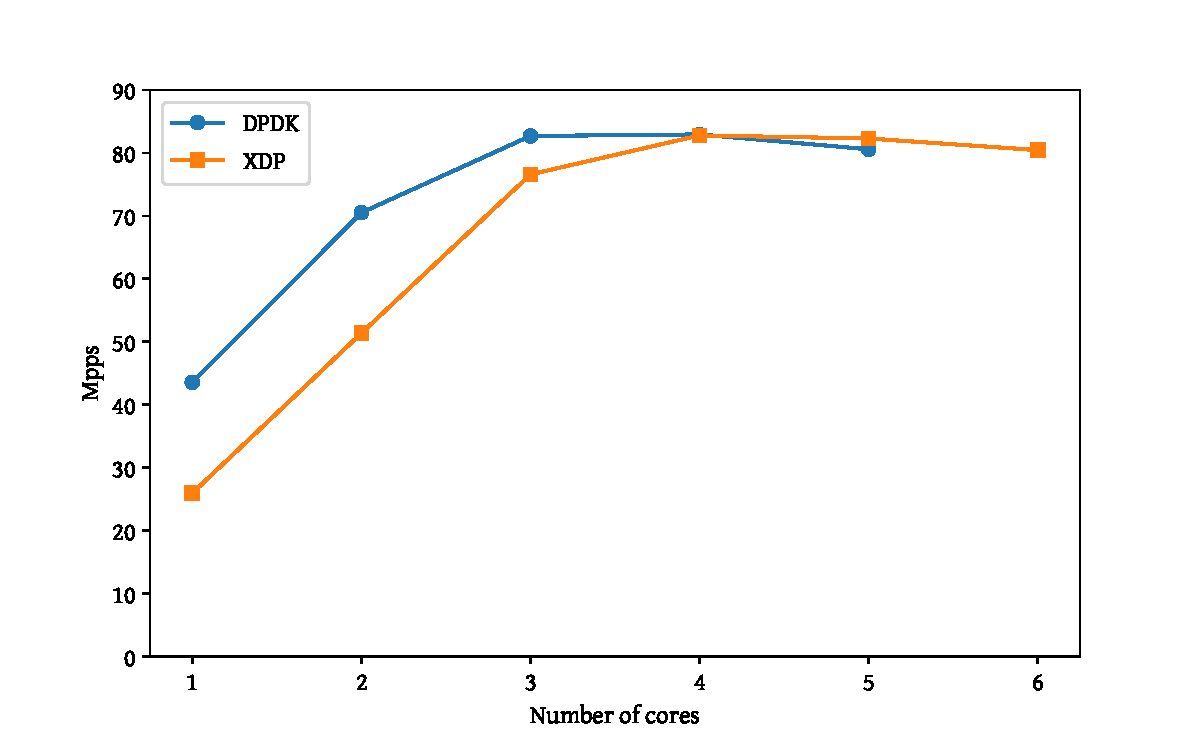
\includegraphics[width=\linewidth]{figures/drop-test.pdf}
\caption{\label{fig:drop-test} Packet drop performance. DPDK uses one core for
  control tasks, which is why it only goes to 5. The slight downward trend at
  above 4 cores is because the performance of our packet generator decreases
  when it has to generate more streams.}
\end{figure}


The hardware performance counters indicate that the global performance
bottleneck is the PCI bus capacity. The reason why DPDK achieves a higher
maximum performance before hitting the limit is that its busy-polling operating
mode allows it to make better use of the available capacity on the bus, while
the NAPI mechanism~\cite{napi} that the Linux kernel (and hence XDP) uses,
intermittently waits for interrupts, which leads to idle periods on the PCI bus.

The figure also shows the performance of the Linux networking stack in two
configurations: One where we use the ``raw'' mode of the \emph{iptables}
firewall module to drop packets, which ensures the earliest possible drop in the
network stack processing; and another where we enable the connection tracking
(\emph{conntrack}) module, which is enabled by default on most Linux
distributions, but which carries a high overhead. These two modes illustrate the
performance span of the Linux networking stack, from 1.8 Mpps of single-core
performance with conntrack, up to 4.8 Mpps in raw mode. It also shows that in
the absence of hardware bottlenecks, Linux performance scales linearly with the
number of cores. And finally, it shows that XDP offers a five-fold improvement
over the fastest processing mode of the regular networking stack, achieving 26
Mpps on a single core.


\subsection{CPU Usage}
\label{sec:cpu-usage}

The CPU usage of the different tested systems, when configured to use a single
core and immediately drop packets, is shown in Figure~\ref{fig:drop-cpu}. The
test varies the offered packet load up to the maximum that each system can
handle on a single core. We then measure the percentage of CPU busy time using
the \texttt{mpstat} system utility.

Since DPDK by design dedicates a full core to packet processing, and uses busy
polling to process the packets, its CPU usage is always pegged at 100\%, which
is the green line at the top of the figure. In contrast, both XDP and Linux
smoothly scale CPU usage with the offered load, with a slightly larger relative
increase in CPU usage at a small offered load level.

\begin{figure}[t]
\centering
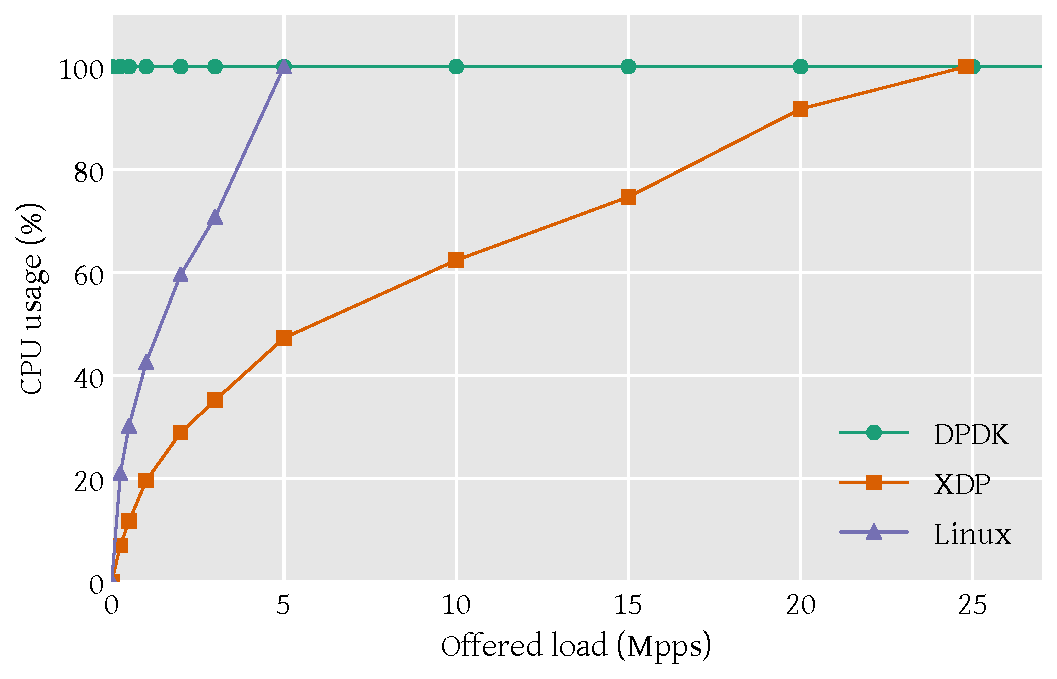
\includegraphics[width=\linewidth]{figures/drop-cpu.pdf}
\caption{\label{fig:drop-cpu} CPU usage in the drop scenario. Each line stops at
  the method's maximum processing capacity. The DPDK line continues at 100\% up
  to the maximum performance shown in Figure~\ref{fig:drop-test}.}
\end{figure}


\subsection{Packet Forwarding Performance}
\label{sec:pack-forw-perf}
Figure~\ref{fig:redirect-test} shows the packet forwarding performance. The
forwarding applications perform a simple Ethernet address rewrite, where the
source and destination address of the incoming packet are swapped before the
packet is forwarded. This is the minimum rewriting that is generally needed for
a real packet forwarding application, so the results represent an upper bound on
forwarding performance. Since XDP can forward packets out the same NIC as well
as out a different NIC (using two different program return codes), we include
both modes in the graph. The DPDK example program only supports forwarding
packets through a different interface, so we only include this operating mode in
the test. Finally, the Linux networking stack does not support this minimal
forwarding mode, but requires a full bridging or routing lookup to forward
packets; this lookup is expensive, and since the other applications don't
perform it, the results are not directly comparable. We instead include the
Linux routing performance in our real-world use case presented in
Section~\ref{sec:fwd-usecase}.

As Figure~\ref{fig:redirect-test} shows, we again see linear scaling the number
of cores up to a global performance bottleneck. The absolute performance is
somewhat lower than for the packet drop case, which shows the overhead of packet
forwarding. We also see that the XDP performance improves significantly when
packets are sent out on the same interface that it was received on, especially
as the number of cores in use increases. This is primarily due to differences in
memory handling: packet buffers are allocated by the device driver and
associated with the receiving interface. And so, when the packet is forwarded
out a different interface, the memory buffer needs to be returned to the
interface that it is associated with, which has some overhead. Work is ongoing
to reduce this overhead.

\begin{figure}[t]
\centering
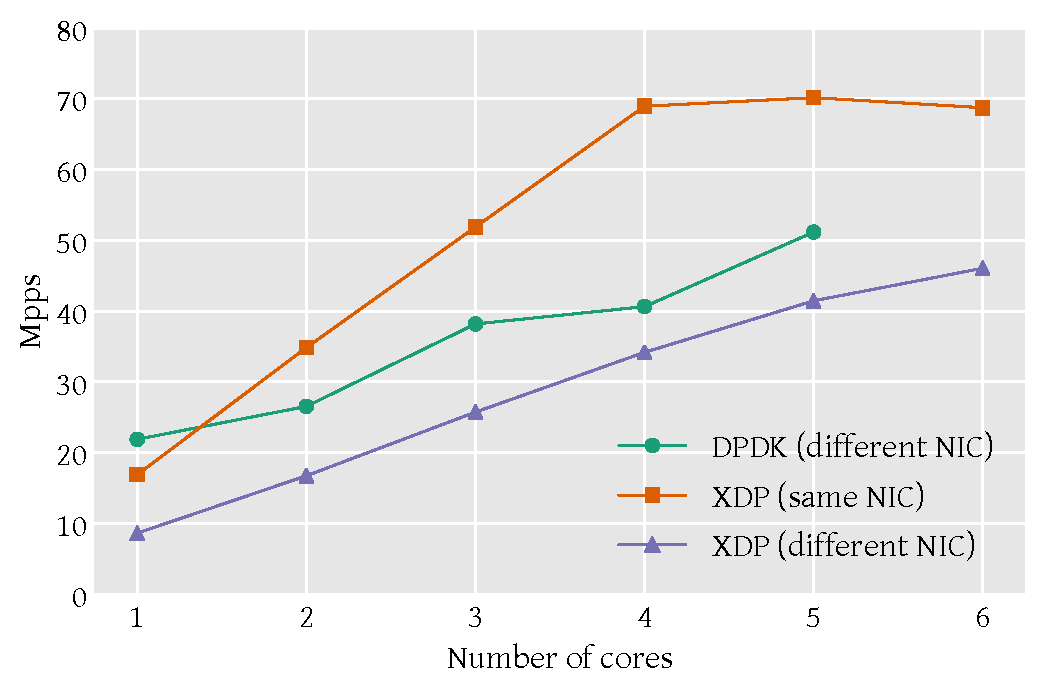
\includegraphics[width=\linewidth]{figures/redirect-test.pdf}
\caption{\label{fig:redirect-test} Packet forwarding performance. At 70 Mpps,
  the same-NIC performance is limited by the PCI bus (since RX and TX on the
  same device means only half the PCI slot bandwidth is available).}
\end{figure}

\subsection{Discussion}
\label{sec:perf-discussion}

As we have seen in the previous sections, XDP achieve significantly higher
performance than the regular Linux networking stack. Even so, for most use cases
XDP doesn't quite match the performance of DPDK. We believe this is primarily
because DPDK has incorporated more performance optimisations at the lowest level
of the code. To illustrate this, consider the packet drop example: XDP achieves
26\,Mpps, which corresponds to 38.4 nanoseconds per packet, while DPDK achieves
43.5\,Mpps, or 22.9 nanoseconds per packet. The difference of 15.5 nanoseconds
corresponds to 56 clock cycles on the 3.6\,Ghz processor in our test machine;
thus, it is clear that every micro-optimisation counts.

Specifically, we identify three areas where the performance of XDP can be
improved: (1) It is possible to eliminate some operations in XDP at the
architectural level, such as DMA map and unmap operations. (2) It is possible to
improve batching of operations, such as packet buffer returns across network
interfaces, and increasing the use of busy polling under heavy load. And (3),
there are some optimisations in the device driver code, such as inlining
function calls, that could be applied specifically to the mlx5 driver. Indeed
other drivers, such as the \emph{i40e} driver for 40\,Gbps Intel cards, show a
smaller performance delta between XDP and DPDK.

Given the above points, we believe it is quite feasible for XDP to close the
performance gap to DPDK completely. In addition, given the fact that this gap is
no longer a matter of orders of magnitude (as is the case between DPDK and the
regular Linux network stack), we believe that given its benefits in terms of
flexibility and integration with the rest of the system, XDP is already a
compelling choice for many use cases. We illustrate some examples of this in the
next section.

\section{Real-world use cases}
\label{sec:usecases}
To show how the various aspects of XDP can used to implement useful real-world
applications, this section gives three examples of such applications. These use
cases have all seen real-world deployment in one form or another, although we
use simplified versions in our evaluation so as to be able to make the code
available.

The first use case shows how XDP's kernel helpers can be used to accelerate
common use cases, using the example of a software router. In the second use
case, we show how an inline Denial of Service (DoS) mitigation application can
be used to protect against attacks directly at the application server. And
finally, the third use case shows how the XDP forwarding mode that sends packets
out the same interface as they arrived on can be used to implement a layer-3
load balancer.

\subsection{The Software Router Use Case}
\label{sec:fwd-usecase}
The Linux kernel contains a full-featured routing table, which includes support
for policy routing, source-specific routing, multipath load balancing, and more.
For the control plane, routing daemons such as Bird or FRR implement a variety
of routing control plane protocols. Because of this rich ecosystem built around
routing on Linux, improving performance of the kernel data plane is desirable;
especially since re-implementing the routing stack in another packet processing
framework carries a high cost.

XDP is a natural fit for this task, especially as it includes a helper function
which makes it possible to perform full routing table lookups directly from XDP.
The result of the lookup is an egress interface and a next-hop MAC address,
which makes it possible for the XDP program to immediately forward the packet if
the lookup succeeds. If no next-hop MAC is known (because neighbour lookup
hasn't been performed yet), the XDP program can instead pass the packet to the
networking stack, which will perform the neighbour lookup, allowing subsequent
packets to be forwarded by the XDP fast path.

To show the performance of this use case, we use the XDP routing example that is
included in the Linux kernel source~\cite{fwd-example} and compare its
performance to the regular Linux networking stack routing. We perform two tests:
one with a single route installed in the routing table and all packets set to
the same destination address. And another where we use a full dump of the global
BGP routing table from \emph{\url{routeviews.org}}, which we import into the
kernel routing table with all next-hop addresses set to the same value. The
routing table dump contains 752,138 distinct routes, and for our tests we
generate 4000 random destination IP addresses to make sure the full lookup table
is exercised.

The performance of this use case is seen in Figure~\ref{fig:router-fwd}. Using
XDP for the forwarding plane improves performance with a factor of 2.5 for a
full table lookup, and a factor 3 for the smaller routing table example. This
makes it feasible to run a software router with a full BGP table at full line
rate on a 10\,Gbps link using only two cores (using a conservative estimate of
an average packet size of 200\,bytes).

\begin{figure}[t]
\centering
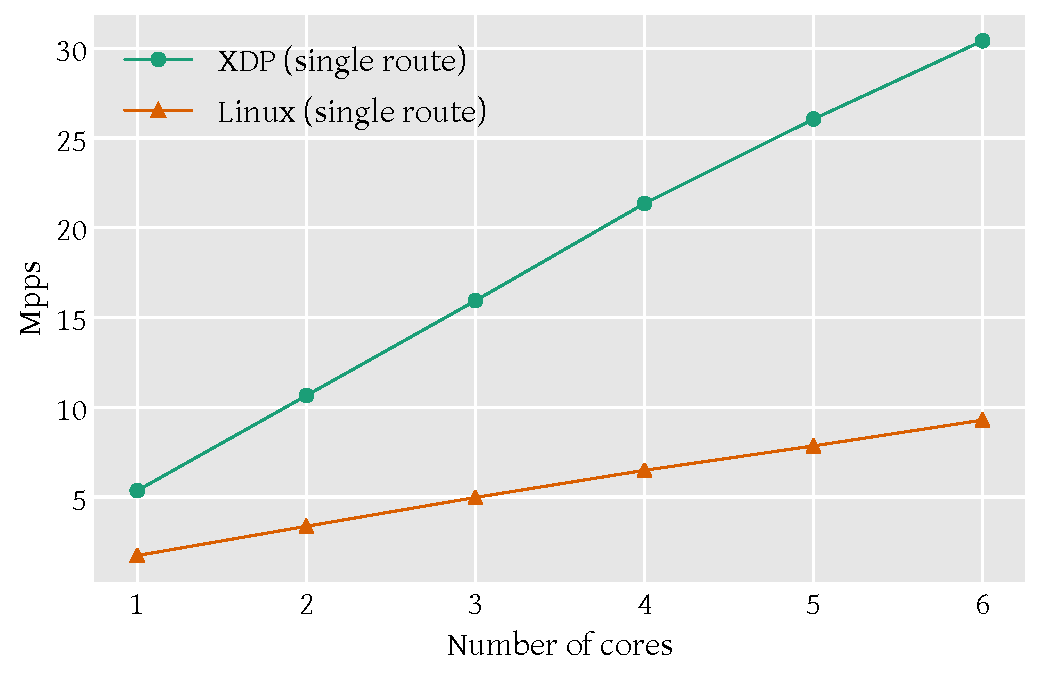
\includegraphics[width=\linewidth]{figures/router-fwd.pdf}
\caption{\label{fig:router-fwd} Software routing performance. Since the
  performance scales linearly with the number of cores, only the results for a
  single core are shown.}
\end{figure}

% See: (calc in benchmarks/bench04_fwd.org). The full-tables vs. single overhead
%  is signficantly larger than the expected overhead (according to Vincent
%  Bernat's measurements)
%  https://vincent.bernat.im/en/blog/2017-performance-progression-ipv4-route-lookup-linux

\subsection{Inline DoS Mitigation}
\label{sec:dos-usecase}
DoS attacks continue to plague the internet, typically in the form of
distributed attacks (DDoS attacks) from compromised devices attached to the
internet. With XDP, it is possible to deploy packet filtering to mitigate such
attacks directly at the application servers, without needing to change the
applications. In the case of a virtual machine deployment, the filter can even
be installed on the hypervisor, and thus protect all virtual machines running on
the host.

To show how this could work, we perform a test modelled on the DDoS mitigation
architecture used by Cloudflare, which uses XDP as the filtering
mechanism~\cite{cloudflare-ddos}. Their Gatebot architecture works by sampling
traffic at servers located in distributed Points of Presence (PoPs), collecting
it centrally for analysis, and formulating mitigation rules based on the
analysis. The mitigation rules take the form of a series of simple checks on the
packet payload, which are compiled directly into eBPF code which is distributed
to the edge servers in the PoPs and executed as an XDP program that will drop
packets matching the rules, while also updating match counters implemented as
BPF maps.

To test the performance of such a solution, we use an XDP program that parses
the packet headers and performs a small number of tests\footnote{A total of four
  tests are performed after the header parsing. For details, see the online
  appendix.} to identify attack traffic and drop it, and uses the CPU redirect
feature to pass all other packets on to the network stack for processing on a
different CPU core. To simulate a baseline application load we use the Netperf
benchmarking tool~\cite{netperf}, which contains a TCP-based round-trip
benchmark, which opens a TCP connection and sends a small payload which is
echoed back from the server, repeating as soon as a reply is received. The
output is the number of transactions per second, which is a good proxy for an
interactive TCP session, such as small remote procedure calls.

We run our experiment on a single core using a single hardware RX-queue.  This
creates the worst possible DoS situation, where good and bad traffic must
compete for the same hardware resources. We apply a baseline load of 35.000 TCP
transactions per second. We then offer an increasing load of small UDP packets
matching our packet filter, which simulates the DoS attack, and measure the
number of TCP transactions achieved as the attack traffic volume increases. We
repeat each experiment four times and report the mean value.

\begin{figure}[t]
\centering
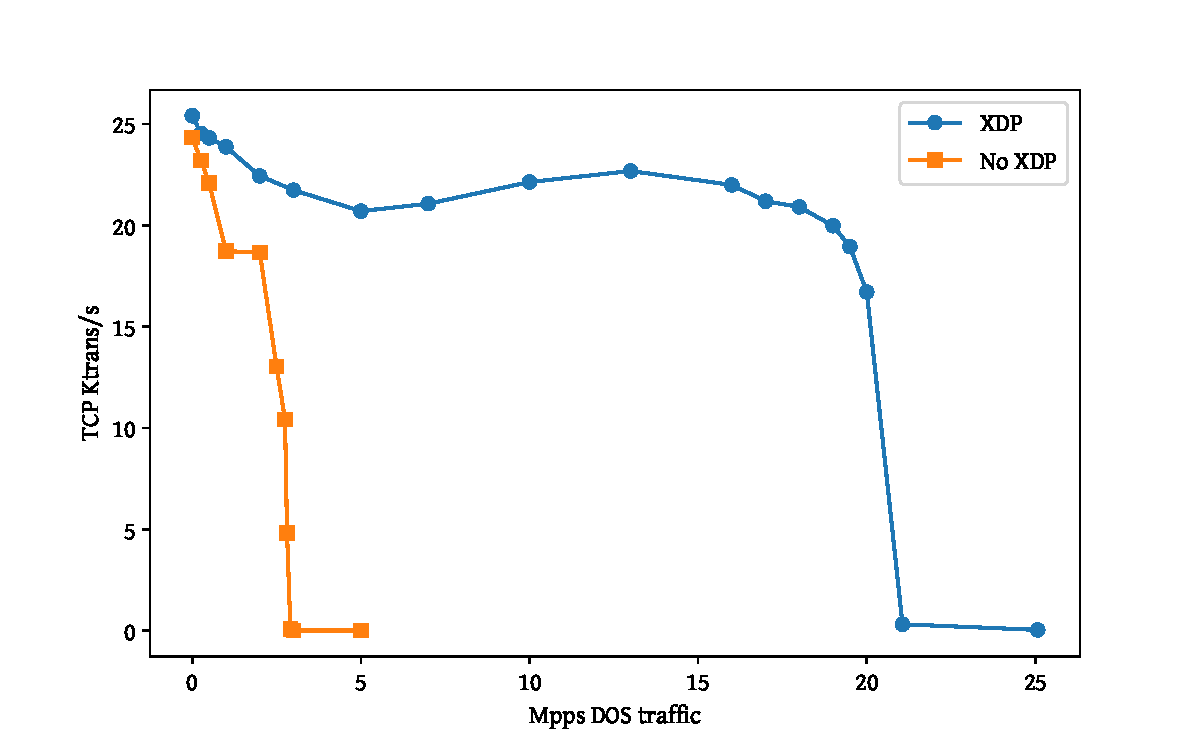
\includegraphics[width=\linewidth]{figures/ddos-test.pdf}
\caption{\label{fig:ddos-results} DDoS performance. Number of TCP transactions
  per second as the level of attack traffic directed at the server increases.}
\end{figure}

The results of this is shown in Figure~\ref{fig:ddos-results}. Without the XDP
filter, performance drops significantly, being halved at 3\,Mpps and effectively
zero at just below 3.5\,Mpps. However, with the XDP filter in place, the TCP
transaction performance is kept high, gradually increasing towards 25.000
transactions per second at 20\,Mpps, after which it drops rapidly. This shows
that effective DDoS filtering is quite feasible to perform in XDP, and
comfortably handles packet rates above 10\,Gbps of DoS traffic (with minimum
packet sizes) on a single CPU core. Deploying DDoS mitigation this way leads to
increased flexibility, since neither application changes, nor additional
hardware is needed.

\subsection{Load Balancer}
\label{sec:load-balancer}
For the load balancer use case, we use the XDP component of the Katran load
balancer~\cite{katran} recently released as open source by Facebook. This works
by announcing a virtual IP address to the world, which is then routed to the
load balancer. At the load balancer, the XDP program hashes the layer-4 packet
header using a stable hashing algorithm, which becomes a destination application
server. The packet is then encapsulated in a new IP header and sent to the
application server, which is responsible for decapsulating it, processing the
request, and replying directly to the originator of the request. This means that
the XDP program can perform the packet encapsulation, and immediately return the
packet out the same interface.

To test this use case, we configure the Katran XDP program with a fixed number
of destination hosts\footnote{We configure one virtual IP per CPU core, with 100
  destination application servers per virtual IP.}, and run it on our test
machine. Once the packets are returned to the network they are simply dropped;
we are only interested in the performance of the load balancer component itself.
This performance is shown in Table~\ref{tbl:load-balancer}, which, as in the
other examples, shows linear scaling with the number of CPUs, and the ability to
saturate a 10\,Gbps link using three CPU cores.

\begin{table}[htbp]
\caption{\label{tbl:load-balancer}Load balancer performance.}
\centering
\begin{tabular}{lcccccc}
  \toprule
  CPU Cores & 1   &  2  &  3  &  4  &  5  &  6  \\
  Mpps & 5.2 & 10.1 & 14.6 & 19.5 & 23.4 & 29.3 \\
\bottomrule
\end{tabular}
\end{table}


\section{Limitations and future work}
\label{sec:limitations}
As we have shown above, XDP offers high performance and can be used to implement
a variety of real-world use cases. However, this does not mean that XDP is a
finished system. On the contrary, as part of the Linux kernel, XDP undergoes
continuing improvement. Some of this development effort goes into softening the
rough edges that are the inevitable result of XDP being incrementally
incorporated into a general purpose operating system kernel. Other efforts
continue to push the boundaries of XDP's capabilities. In this section we give a
(non-exhaustive) overview of the efforts in both areas of development. These
include: User experience and debugging; driver support; performance
improvements; QoS and better handling of rate transitions; and acceleration of
transport protocols. The following subsections discuss each of these issues in
turn.

\subsection{User Experience and Debugging}
\label{sec:user-exper-debugg}
Since an XDP program runs in the kernel, the debugging tools available to a
regular userspace program are not generally applicable. Instead, the debugging
and introspection features included in the kernel can be applied to XDP (and
other eBPF) programs as well. These tools include tracepoints and
kprobes~\cite{kernel-tracing} as well as the performance counts that are part of
the \emph{perf} subsystem~\cite{perf}. However, developers who are not familiar
with the kernel ecosystem and ``just wants to write packet processing programs''
can find this ecosystem of kernel-specific tools a limitation, as others have
noted~\cite{miano2018creating}. To ease the transition, a wide variety of tools
exist, including the BPF Compiler Collection~\cite{bcc}, the \emph{bpftool}
introspection program~\cite{bpftool} and the \emph{libbpf} library of utility
functions~\cite{libbpf}. These have already seen significant improvements since
their inception, but more work is needed in this area.

Another area that sees continual improvement is the eBPF program verifier. The
primary focus of the verifier is naturally to ensure the correctness and safety
of the programs being loaded into the kernel. As such, a conservative approach
is taken, where the verifier will reject any program that it cannot prove is
correct. This can lead to false negatives, where correct programs are rejected.
In addition, the restrictions on the program structure initially imposed by the
verifier, such as the lack of support for function calls and loops, have been
more limited than strictly necessary, in the interest of ensuring safety first.
To improve upon this situation, there is ongoing to teach the verifier to
recognise more correct programs that were previously rejected as invalid, and
the error messages reported by the verifier have been made friendlier, to make
it easier for developers to change their code to avoid verification errors. In
addition, support for function calls in eBPF has recently been added, and the
addition of support for bounded loops is planned. Efficiency improvements that
will allow the verifier to operate on much larger programs are also being worked
on.

\subsection{Driver Support}
\label{sec:driver-support}
Each device driver needs to add support for running XDP programs, by supporting
an API exposed by the core networking stack. Support is continuously being added
to more and more drivers,\footnote{At the time of writing Linux 4.17 has XDP
  support in 12 different drivers, including the most popular high-speed network
  adapters. An updated list of supported drivers is included in
  \url{http://cilium.readthedocs.io/en/latest/bpf}.} but at the time of writing,
some care is still needed when selecting hardware to use with XDP. However,
since XDP is integrated into the kernel device driver model, it imposes no
particular capability constraints on the hardware, which means that full support
in all drivers is possible; and indeed we believe that is how this limitation
will eventually be resolved.

As the XDP system has evolved, the need to keep the changes required in drivers
to support XDP to a minimum has become increasingly clear, and some steps have
been taken in this direction. For instance, support for new targets can be added
to the redirection action without any changes needed from the drivers. Finally,
the Genereic XDP feature~\cite{generic-xdp} makes it possible to run XDP
programs at reduced performance even if the networking driver lacks the proper
support, by moving execution into the core networking stack.

\subsection{Performance Improvements}
\label{sec:improvements-napi}
As we discussed in Section~\ref{sec:perf-discussion}, there is still a
performance gap between XDP and DPDK in some use cases. Efforts to improve this
are ongoing, which includes micro-optimisations of driver code as well as
changes to the core XDP code to avoid unnecessary operations where possible, and
otherwise amortise the costs through improved batching of operations.

One particular area that needs improvement is the NAPI mechanism, which
selectively switches between interrupt-based packet processing and polling. This
is insufficient to mitigate the large number of interrupts that happen at high
packet rates, which means that in some cases it would be beneficial to switch to
a full busy polling mode, where one or more full CPU cores are dedicated to
polling the hardware receive rings and process packets as soon as they appear.
There have been some efforts to selective switch a network adapter to busy
polling mode, which has shown promising results~\cite{dumazet17:_busyp}. As we
noted in Section~\ref{sec:perf-discussion}, we believe that integrating this
work with XDP, will, along with the other performance optimisations mentioned
above, make it possible to reach raw packet processing performance at least
equal to that of DPDK.

\subsection{QoS and Rate Transitions}
\label{sec:handl-rate-trans}
Currently, XDP does not implement any mechanism for supporting different Quality
of Service (QoS). Specifically, an XDP program receives no backpressure when
attempting to forward packets to a destination that has exhausted its capacity.
This limitation can be exasperated when joining networks with different speeds
or other mismatched network characteristics.

While QoS is lacking from XDP, the Linux kernel networking stack features
best-in-class Active Queue Management (AQM) and packet scheduling
algorithms~\cite{good-bad-wifi}. While not all of these features are a good fit
for the XDP architecture, we believe that selectively integrating features in
this area from the networking stack into XDP is an opportunity to provide
excellent support for QoS and AQM in XDP in a way that can be completely
transparent to the packet processing applications themselves. We are planning to
explore this further in the future.

\subsection{Accelerating Transport Protocols}
\label{sec:accel-transp-prot}

With XDP we have shown how high-speed packet processing can be integrated
cooperatively into the operating system to accelerate processing while making
use of existing features of the operating system where it makes sense. XDP
focuses on stateless packet processing, but extending the same model to stateful
transport protocols such as TCP would provide many of the same performance
benefits to applications that require reliable (and thus stateful) transports.
There has been some initial discussion of this in the community~\cite{txdp};
expanding this presents an exciting opportunity for expanding the scope of the
XDP system.

\section{Conclusions}
\label{sec:conclusion}
We have presented XDP, a system for safely integrating high-speed programmable
packet processing directly in the Linux kernel. This represents an alternative
solution to all-or-nothing kernel bypass solutions, which makes it easier to
integrate the packet processing with normal applications.

Our evaluation has shown that XDP achieves raw packet processing performance of
up to 25 million packets per second on a single CPU core. We have also
demonstrated three examples of real-world use cases that can be implemented with
XDP: Inline DDOS mitigation, layer-3 forwarding, and layer-4 load balancing.

XDP continues to be actively developed by the Linux community, and we believe
that it offers a compelling alternative to other high-speed packet processing
frameworks, especially where integrating with existing systems and applications
is important.

\bibliographystyle{ACM-Reference-Format}
\bibliography{xdp}

\end{document}
